\chapter{Hybrid Eulerian-Lagrangian Vortex Particle Method}

% Summarize the sections. : domain decomposition, coordinate systems assosciated to each
% subdomains, and the coupled evolution of the hybrid method.
% Reference to the literatures: Cottet and others, stock and daenick
% We use approach of stock based on the phd research of daeninck

The \printAcron{Hybrid Eulerian-Lagrangian Vortex Particle Method}{HELVPM} is a domain decomposition method, where the Eulerian method and the Lagrangian method solves different regions of the fluid. The domain decomposition method simply splits the domain of interest and uses appropriate method in each domain. The Eulerian formulation will be used at the near-wall region, where we need proper description of the vorticity generation at the boundary, and the Lagrangian formulation is used away from the body, where we only need to evolve the vorticity field. Figure \ref{fig:domainDecomposition} shows the decomposition of the domain in the gridded and the non-gridded region.

Several studies have already been done: Cottet and Koumoutsakos (2000a)\cite{Cottet2000a}, Guermond and Lu (2000) \cite{Guermond2000a} simulated the advection dominated flows; Ould-Salhi et al. (2001) \cite{Ould-Salihi2001a} blended the finite difference and vortex method together; Winckelmans et al. (2005a) \cite{Winckelmans2005} investigated the trailing vorticies; Daeninck (2006) \cite{Daeninck2006} used a simplified coupling strategy, coupling Vortex Particle Method and Finite Diference Method; Stock (2010) \cite{Stock2010a} expanded Daeninck's strategy, coupling Vortex Particle Method and Finite Volume Method and modeled a 3-D rotor.

	\section{Convectional coupling strategy}
	
	When investigating these works, we see that not all domain decomposition methods are the same. The main difference between the methods is their coupling strategies. Most works employ the\textit{ Schwartz alternating method} to couple the vortex particle method and the grid solver. The Schwartz alternating method (or sometimes referred to as Schwartz iterative method), couples the vortex particle method and the grid solver by iteratively determining the boundary condition such that the stream functions in both domains, $\psi_L$ and $\psi_E$ in $\Omega_L$ and $\Omega_E$ respectively, match at the overlap region $\Omega_E-\Omega_L$, shown in Figure \ref{fig:domainDecomposition}. The summary of a single iteration of the Schwartz alternating method is as follows:
	
		\begin{itemize}
		\item Determine the Eulerian boundary condition, the stream function $\psi_{\Gamma_E}$ at the Eulerian boundary $\Gamma_E$, extracted from the Lagrangian stream function $\psi_L$ in the Lagrangian subdomain $\Omega_L$.
		\item Solve for the stream function $\psi_E$ in the Eulerian subdomain $\Omega_E$ with the new boundary condition $\Gamma_E$.
		\item Determine the Lagrangian condition, the stream function $\psi_{\Gamma_L}$ at the Lagrangian boundary $\Gamma_L$, extracted from the Eulerian stream function $\psi_E$ in the Eulerian subdomain $\Omega_E$.
		\item Solve the stream function $\psi_L$ in the Lagrangian subdomain with the boundary conditions $\psi_{\Gamma_L}$ at the Lagrangian boundary $\Gamma_L$.
		\end{itemize}
	
	This procedure is iterated until the stream functions of both domains converge \cite{Ould-Salihi2001a}. Once the stream function is determined in both the domains, the velocity field can be obtained. Using the velocity field, we can evolve the vorticity field in the Lagrangian subdomain.

	As we realized now, the downside to this procedure is that we have to solve the stream function in both $\Omega_E$ and $\Omega_L$ iteratively, until we converge to a solution. This makes the computation very expensive, especially when we are dealing with large numbers of vortex particles. Therefore, for this project, we are using the coupling technique that is based on the research work of Daeninck (2006) \cite{Daeninck2006} and Stock (2010) \cite{Stock2010a}. However we had to perform a modification to their scheme to ensure that the total circulation of the Lagrangian domain is conserved at all times.
	
		\begin{figure}[!t]
			\centering
			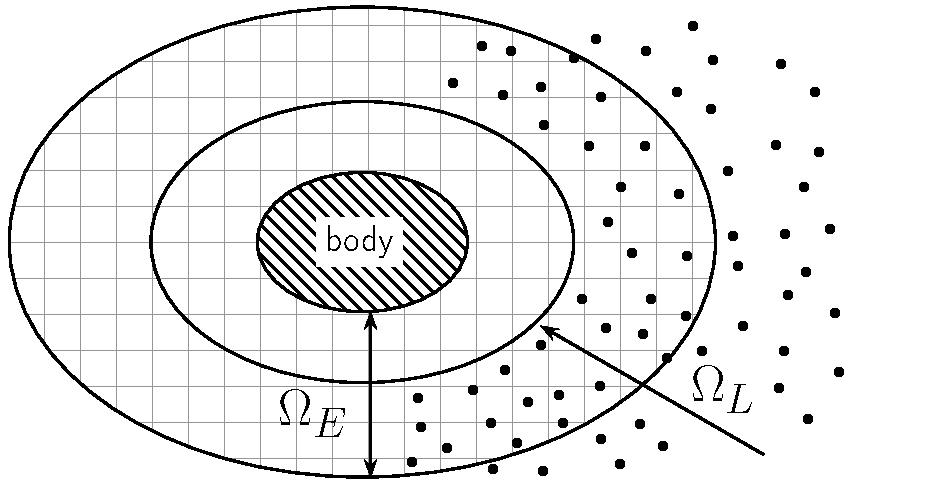
\includegraphics[width=0.6\linewidth]{figures/introduction/domainDecomposition_typical_type2.pdf}
			\caption{Standard domain decomposition using Schwartz iteration for coupling the two methods. Eulerian subdomain $\Omega_E$ (near the body), and Lagrangian subdomain $\Omega_L$ (away from the body). Figure is based on Guermond (2000) \cite{Guermond2000a}}.
			\label{fig:domainDecomposition}
		\end{figure}

	\section{Simplified coupling strategy}

	The simplified coupling strategy was first demonstrated by Daeninck \cite{Daeninck2006}. Daeninck showed that it is possible to coupled the Lagrangian and the Eulerian method without the use of Schwartz iterative method. The basic algorithm consists of solving the vortex method in the full fluid domain using a relatively coarse resolution on the near-wall region. Then we use the grid solver in the near-wall region to capture the detailed features of the boundary layer and transfer the vorticity field in this region to the vortex particles, figure \ref{fig:domainDecomposition_daenick}. Therefore, the grid solver essentially acts as the correction for the under-resolved regions of the Lagrangian method. The functionality of this strategy has been demonstrated by Daeninck and was found to be significantly faster than the Schwartz coupling strategy. The features of the simple coupling strategy can summarized as follows:

		\begin{itemize}
		\item Eulerian method is used to resolve the near-wall region, at the Eulerian subdomain $\Omega_E$, enabling it to capture important features of the boundary layer (such as flow separation) with great accuracy.
		
		\item Lagrangian method is used to capture the wake, at the Lagrangian subdomain $\Omega_L$, and to efficiently evolve the wake.
		
		\end{itemize}


		\item The accurate solution of the Eulerian subdomain is transfered to the Lagrangian subdomain according to the coupling algorithm of Daeninck \cite{Daeninck2006} and Stock \cite{Stock2010a}. In addition to their algorithm, a correction in done on the transfer to ensure conservation of circulation.
		
		\item The boundary conditions for the Eulerian subdomain are retrieved from the Lagrangian subdomain.

		\begin{figure}[!t]
			\centering
			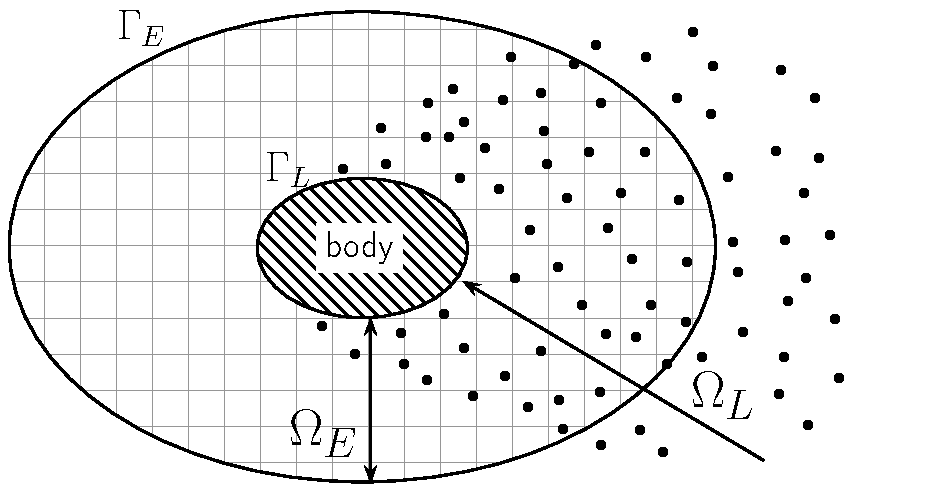
\includegraphics[width=0.6\linewidth]{figures/introduction/domainDecomposition_daenick_type2.pdf}
			\caption{Modified domain decomposition \underline{without} Schwartz alternating method. Lagrangian subdomain extends up to the surface of the body. Figure is based on Daeninck (2006) \cite{Daeninck2006}.}
			\label{fig:domainDecomposition_daenick}
		\end{figure}

		\subsection{Decomposition of the domain}
			% Summary of the terminology
			% Schematic of the domain decomposition: general, and close-up.
	
	%		\subsection{Coordinate Systems}
	%			% Coordinate system: local to global transformation.
	%			% summarize: coordinates systems of panels, lagrangian, eulerian
	%			% how is the body defined? How it the problem constructed? 

	\section{Evolution of the Hybrid Method}
	
	The algorithm to the \printAcron{Simple Coupling Strategy}{SCS} follows from Daeninck's doctoral thesis, \cite{Daeninck2006}. Figure \ref{fig:flowchart_simpleCoupling} shows the overview to the algorithm and can be summarized as follows:

		\begin{enumerate}
		\item \textbf{Correct Lagrangian:} Use the solution of the Eulerian subdomain $\Omega_E$ (in the near-wall region) to correct the solution of the Lagrangian subdomain $\Omega_L$, that is overlapping the Eulerian subdomain, ensuring that the \textit{circulation is conserved}.  
		
		\item \textbf{Evolve Lagrangian:} With the modified solution, evolve the Lagrangian solution from time step $t_n$ to next time step $t_{n+1}$.
		
		\item \textbf{Determine Eulerian boundary conditions:} Use the Lagrangian solution of time $t_{n+1}$ to determine the boundary conditions of the Eulerian subdomain at $t_{n+1}$.
		
		\item \textbf{Evolve Eulerian:} With the boundary condition, evolve the Eulerian solution from $t_n$ to $t_{n+1}$.
		\end{enumerate}
	
	This is the basic approach for coupling the Eulerian method in the Eulerian subdomain $\Omega_E$ with the Lagrangian method in the Lagrangian subdomain $\Omega_L$ without the iterative Schwartz algorithm. 
	
	Furthermore, the SCS handles the Lagrangian boundary condition differently from the classic hybrid method. Typically during the evolution process of the Lagrangian subdomain, the shedding of the vorticity is also defined in the Lagrangian method. However, in our coupling strategy, the Lagrangian method is under-resolved at the boundary and cannot be used to resolve the vorticity flux at the body. Instead, we use the Eulerian method to resolve the boundary, and the Eulerian method acts as the vorticity generator for the Lagrangian method. However, there are some assumptions that we must satisfy, for this coupling strategy to be valid:

	\begin{itemize}
	\item At $t_n$ before the evolution of both method to $t_{n+1}$, the Lagrangian solution matches Eulerian solution at the boundary of the near-wall region.
	\item After the evolution to $t_{n+1}$, the deviation of the Lagrangian solution (due to lack of vorticity flux at Lagrangian boundary), should be minimal.
	\item Even though the Lagrangian subdomain is under-resolved in the near-wall region, it should be able to provide accurate boundary conditions for the Eulerian external boundary.
	\end{itemize}
	
	\begin{figure}[!t]
		\centering
		\begin{tikzpicture}
			[node distance=.8cm, start chain=going below,]
			\node[punktchain, join] (correct) {Correct the \\Lagrangian subdomain};
		    \node[punktchain, join] (evolveL) {Evolve the Lagrangian solution};
		    \node[punktchain, join] (bcE)     {Determine the \\Eulerian boundary conditions};
		    \node[punktchain, join] (evolveE) {Evolve the Eulerian solution};
		\end{tikzpicture}
		\caption{Flowchart of the simple coupling strategy. The flowchart shows the procedure to evolve both methods from $t_n$ to $t_{n+1}$.}
		\label{fig:flowchart_simpleCoupling}
	\end{figure}




% Summarize daenincks approach:
	% Methodology, algorithm
	% Domain decomposition
% Summarize stock's approach:
	% Methodology, algorithms
	% Resulted domain decomposition.